%%%Slides
  \begin{figure} \centering  % [h!]  [!ht]
    \caption{ ~Simulated dynamics from a SIR model of stock investors}
    \label{fig:sir_simulate}
    \centerline{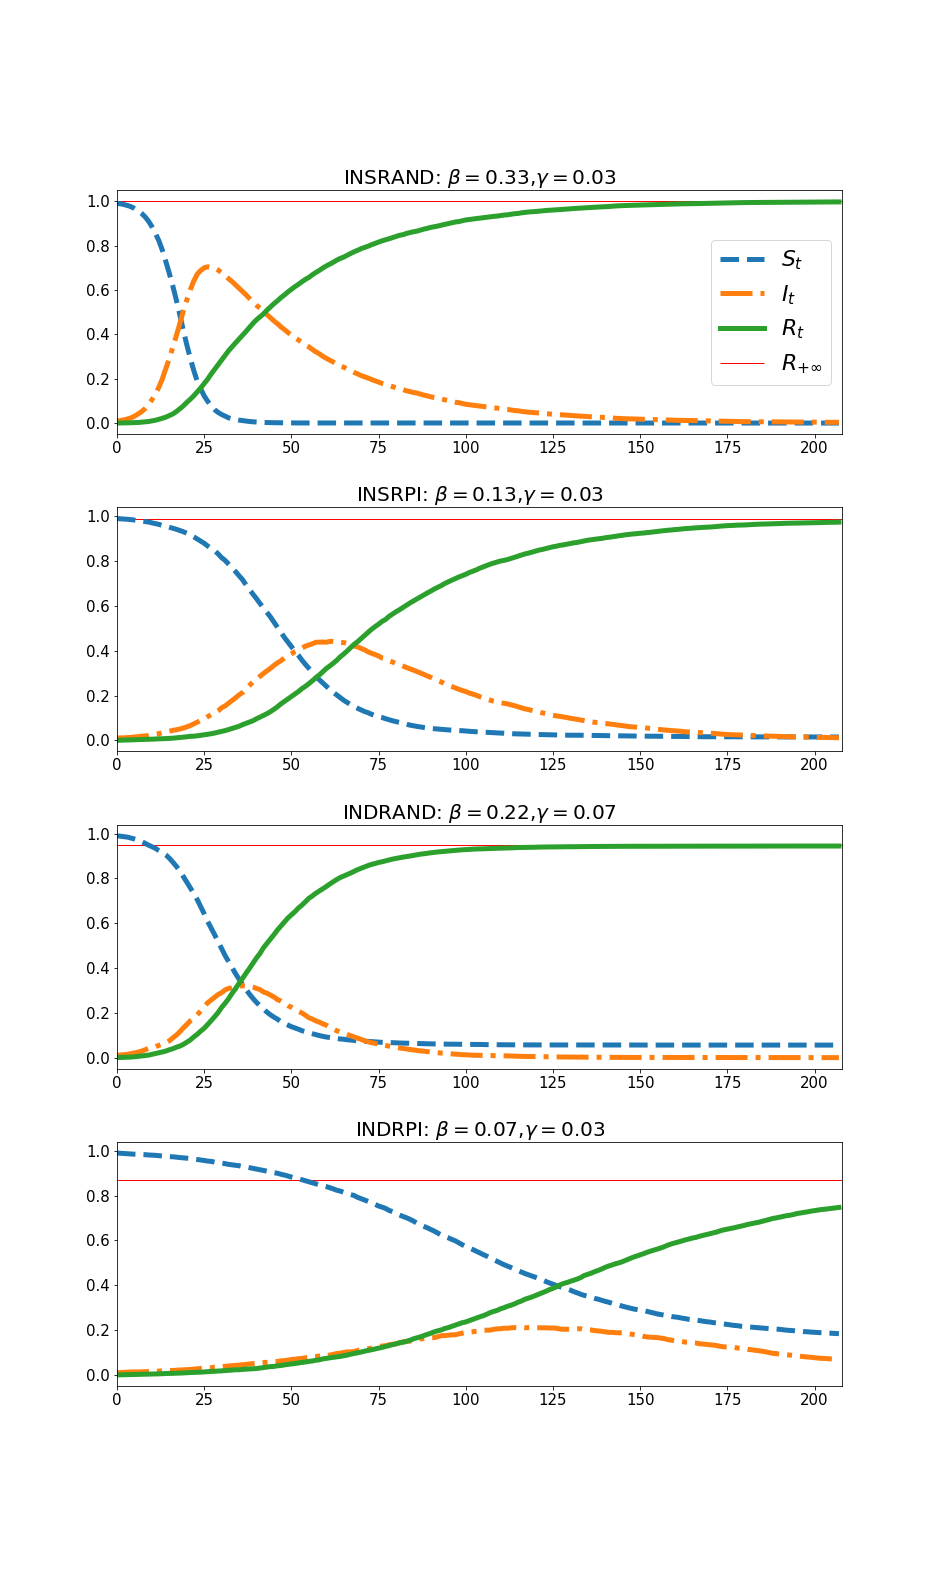
\includegraphics[width=0.85\textwidth,height=0.85\textheight]{./figures/sir_simulate}}
    \begin{flushleft}
      {\footnotesize Note: This graph plots the simulated paths of populations in different compartments in a SIR model of stock investors, as described in \cite{shiller1989survey}. We use the median estimates of the infection rate $\beta$ and recovery rate $\gamma$ for four samples: institutional investors for a randomly selected stock (INSRAND), institutional investors for a rapidly rising stock (INSRPI), individual investors for a random stock (INDRAND), and individual investors for a rapidly rising stock (INDRPI). The horizontal thin solid line corresponds to the limiting size of compartment of $R$ in the long run. The simulation is done with the Python library \href{https://ndlib.readthedocs.io/en/latest/}{``NDlib''}, for details, see the companion \href{https://github.com/llorracc/EpiExp/blob/master/SIR_Ndlib.ipynb}{Jupyter Notebook}. }
    \end{flushleft}
  \end{figure}
